\begin{frame}[t]
 \frametitle{Fundamental Symmetries in Physics}
 \begin{block}{Continuous global symmetries}
  \begin{itemize}
   \item \alert{Translational} (time and space) and \alert{rotational} symmetry
   \item<2> Also, \alert{phase of wave functions} in quantum mechanics
  \end{itemize}
 \end{block}
 \begin{block}{Conserved quantities}
  \begin{itemize}
   \item \alert{Energy and momentum} due to translational symmetry
   \item \alert{Angular momentum} due to rotation symmetry
   \item<2> \alert{Charge conservation} due to global change of phase
   \begin{center}
    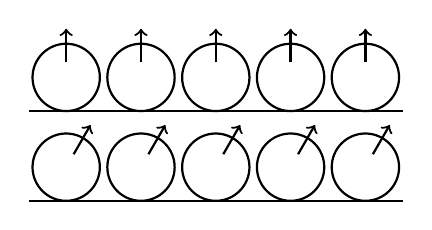
\begin{tikzpicture}[thick,scale=0.95]
     % Definitions
     \def\r{0.45}
     \def\off{0.2}
     \def\len{0.45}
     % Line and circles
     \foreach \y/\mycos/\mysin in {0/0/1,-1.2/0.5/0.866} {
      \draw (0,\y) -- (5,\y);
      \foreach \x in {0.5,1.5,2.5,3.5,4.5} {
       \draw (\x,\y+\r) circle (\r);
       \draw[->] (\x+\off*\mycos,\y+\r+\off*\mysin) -- (\x+\off*\mycos+\len*\mycos,\y+\r+\off*\mysin+\len*\mysin);
      };
     };
    \end{tikzpicture}
   \end{center}
  \end{itemize}
 \end{block}
\end{frame}
